%%%%%%%%%%%%%%%%%%%%%%%%%%%%%%%%%%%%%%%%%%%%%%%%%%%%%%%%%%%%%%%%%%%%%%
% Lớp 12 | Ứng dụng đạo hàm để khảo sát hàm số | Giá trị lớn nhất và giá trị nhỏ nhất của hàm số
% Dạng 2D1?3-3: Sử dụng các đánh giá, bất đẳng thức cổ điển
% Số câu: 3  (sinh tự động bởi tach_cau.py; từ nay thầy sửa trực tiếp file này)
%%%%%%%%%%%%%%%%%%%%%%%%%%%%%%%%%%%%%%%%%%%%%%%%%%%%%%%%%%%%%%%%%%%%%%

%%%%%%%%%%%%%%%% TRẮC NGHIỆM 4 PHƯƠNG ÁN %%%%%%%%%%%%%%%%

% nguồn: Phan1_Lop_12_Dai_so_Chuong_1
\begin{ex}%[2D1H3-3]%[ma:c914238c]
	Cho  hàm số $y=f(x)$ liên tục trên $\mathbb{R}$ và có đồ thị như hình dưới
	\begin{center}
		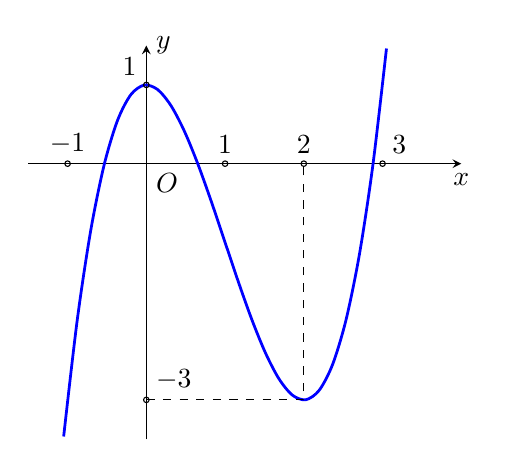
\begin{tikzpicture}[>=stealth]
			\draw[->] (-1.5,0) --(0,0) node[below 
				 right]{$O$} -- (4,0)
				node[below]{$x$}; 
			\draw[->](0,-3.5)--(0,1.5) 
				node[right]{$y$}; 
			 \draw[smooth,blue,line width=1]
				plot[domain=-1.05:3.05] 
				(\x,{(\x)^(3)-3*(\x)^(2)+1}); 
			\draw[dashed] (0,-3)  node[left]{} -- (2,-3) --
				 (2,0) node[above]{$2$};
			\draw (0,-3) node[above right]  {$-3$} circle (1pt);
			 \draw (2,0) circle (1pt);
			\draw (1,0)  node[above] {$1$} circle (1pt);
			\draw (0,1)  node[above left] {$1$}circle (1pt);
			\draw (3,0) node[above  right] {$3$}circle (1pt);
			\draw (-1,0)  node[above] {$-1$}circle (1pt);
		\end{tikzpicture}
	\end{center}
	Tìm giá trị lớn nhất của hàm số $y=f^2(x)+3$ trên  đoạn $[0; 2]$.
	 \choice
		{\True  $12$}
		{$13$} 
		 {$2$}
		{$9$} 
	 \loigiai{
		Đặt $g(x)=f^2(x)+3$. Từ đồ thị đã cho ta  có $\exists x_0 \in(0; 1)$ để $f\left(x_0\right)=0$.
		Với $x\in [0;2]$  thì
		\begin{eqnarray*}
			-3 \leq f(x) \leq 1 &\Rightarrow&  0 \leq f^2(x) \leq 9\\
			&\Rightarrow& 3 \leq  f^2(x)+3 \leq 12\\
			&\Rightarrow& 3 \leq g(x)  \leq 12\\
			&\Rightarrow& \max _{[0; 2]} g(x)=12  \text {khi } f(x)=-3\\
			&\Rightarrow& x=2  \in[0; 2].
		\end{eqnarray*}
	 }
\end{ex}

% nguồn: Phan1_Lop_12_Dai_so_Chuong_1
\begin{ex}%[2D1H3-3]%[ma:bfeb3565]
	Giá trị lớn  nhất của hàm số $y=\sqrt{16-x^2}$ là
	\choice 
		{$16$} 
		 {\True $4$}
		{$0$} 
		 {$1$}
	\loigiai{ 
		Ta  có $y=\sqrt{16-x^2}\le 4$.\\
		Dấu \lq\lq =\rq\rq~xảy ra khi $x=0$.\\ 
		 Vậy $\max\limits_{[-4;4]}y=4$.
	} 
\end{ex}


%%%%%%%%%%%%%%%% TRẢ LỜI NGẮN %%%%%%%%%%%%%%%%

% nguồn: Phan2_Lop_12_Dai_so_Chuong_1
\begin{bt}%[2D1V3-3]%[ma:91a60ee4]
	Hàm số $y = (x + m)^3 + (x + n)^3 - x^3$ (tham số là $m, n$) đồng biến trên $(-\infty; +\infty)$. Biết giá trị nhỏ nhất của biểu thức $P =  4\left(m^2 + n^2\right) - 2m - 2n$ là $-\dfrac{a}{b}$, với $\dfrac{a}{b}$ là phân số tối giản. Tính $a+b$.
	\shortans{5} 
	 \loigiai{
		Ta có $y' = 3(x + m)^2 +  3(x + n)^2 - 3x^2 = 3\left[x^2 + 2(m + n)x + n^2 + m^2\right]$.\\
		Để hàm số đồng biến trên $(-\infty; +\infty)$ thì $y' \ge 0,\ \forall x \in \mathbb{R} \Leftrightarrow \Delta' = (m + n)^2  - (m^2 + n^2) \le 0 \Leftrightarrow mn \le 0$.\\
		Mặt khác,  ta có
		\begin{eqnarray*}
			P &=& 4\left(m^2 + n^2\right) - 2m - 2n = 4(m + n)^2 - 2(m + n) -  8mn\\
			&=& \left[2(m + n) - \dfrac{1}{2} \right]^2  + (-8mn) - \dfrac{1}{4} \ge -\dfrac{1}{4}.
		\end{eqnarray*}
		Suy ra $Min\,P =  -\dfrac{1}{4} \Leftrightarrow \heva{&n = 0, m = \dfrac{1}{4}\\&m = 0, n = \dfrac{1}{4}}$.\\
		Do đó $a=1$, $b=4$.  Vậy $a+b=5$.
	} 
\end{bt}
